\documentclass[11pt]{article}

\usepackage{../algebra}

\begin{document}

\coverpage{4}

% hw problem 1 -----------------------------------------------------------------

\begin{exercise}{55}{21}
    \problem{
        If $A, B$ are subgroups of $G$ such that $b^{-1} A b \subset A$ for all $b \in B$, show that $AB$ is a subgroup of $G$.
    }
    \proof{
        Our task is to show that $AB \leq G$.
        Note that $AB := \{ ab \mid a \in A, b \in B \}$.
        We are also given the conditions that $A,B \leq G$ and $b^{-1} A b = \{ b^{-1} a b \mid a \in A \} \subset A$ for all $b \in B$.
        We get associativity for free and we can quickly deduce that $e \in AB$ since $e \in A, B$ and $e = ee \in AB$. \parspace
        We now show that $AB$ is closed under the group operation in $G$.
        Pick any $x, y \in AB$ then $x = a_1 b_1$ and $y = a_2 b_2$ for some $a_1, a_2 \in A$ and $b_1, b_2 \in B$.
        Then $xy = a_1 b_1 a_2 b_2 = b_1 b_1^{-1} a_1 b_1 a_2 b_2$ where the existence of $b_1^{-1}$ is guaranteed since $G$ is a group.
        But then $b_1^{-1} a_1 b_1 \in A$ so let $b_1^{-1} a_1 b_1 = a_3 \in A$.
        Then we have $xy = b_1 a_3 a_2 b_2$.
        Setting $a_4 = a_3 a_2$ ($a_4 \in A$ by closedness), we get $xy = b_1 a_4 b_2$.
        Again since $G$ is a group, we can say that $ b_1 a_4 b_2 = b_1 a_4 b_1^{-1} b_1 b_2 = (b_1^{-1})^{-1} a_4 b_1^{-1} b_1 b_2$.
        Then let $a = (b_1^{-1})^{-1} a_4 b_1^{-1}$ (a member of $A$ by our assumed property) and $b = b_1 b_2$ (a member of $B$ by closedness) and then we have $xy = ab$ where $a \in A, b \in B$.
        Thus $cd \in AB$. \parspace
        As the final step torwards proving $AB \leq G$, we must verify that every element has an inverse in $AB$.
        Fix any $x = ab \in AB$, we wonder if $x^{-1} = (ab)^{-1} \in AB$.
        Certainly $(ab)^{-1} \in G $ and $(ab)^{-1} = b^{-1} a^{-1} = b^{-1} a^{-1} b b^{-1}$ by properties of $G$.
        But then we know $b^{-1} a^{-1} b \in A$ (since $a^{-1}$ is an element of $A$ so the property applies).
        Letting $b^{-1} a^{-1} b = a' \in A$ we have $x^{-1} = a' b^{-1}$ which must be a member of $AB$ since $a' \in A$ and $b^{-1} \in B$ (since $B$ is subgroup).
        Therefore, $AB$ is a subgroup of $G$.
    }
\end{exercise}

% hw problem 2 -----------------------------------------------------------------

\begin{exercise}{65}{19}
    \problem{
        Find all the distinct conjugacy classes of $S_3$.
    }
    \proof{
        Our goal is to find all the distinct conjugacy classes of $S_3$.
        Recall that $S_3 = \{ id, (12), (13), (23), (123), (321) \}$ and note that $(123)^{-1} = (321)$ (see Figure \ref{fig:123inv} for proof).
        Given $f,g \in S_3$ we have $f \sim g$ ($f$ and $g$ are conjugate) if there exists some $h \in G$ such that $g = h^{-1} f h$.
        The textbook also notes that $\sim$ is an equivalence relation. \parspace

        \begin{figure}[h]
            \centering
            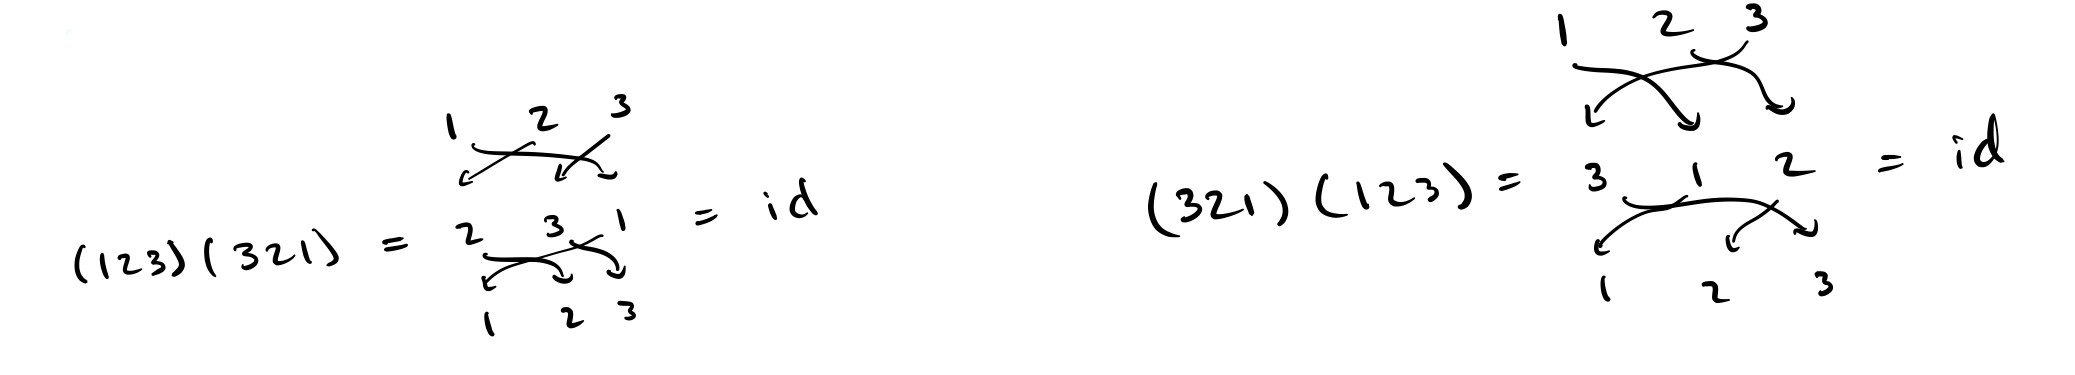
\includegraphics[width=0.95\textwidth]{img/123inv}
            \caption{Showing $(123)^{-1} = (321)$}
            \label{fig:123inv}
        \end{figure}

        First, we show that $\{ id \}$ is a conjugacy class.
        Since $\sim$ is an equivalence relation, we necessarily have $id \sim id$.
        Now pick $f$ a member of the conjugacy class of $id$.
        Then $id = g^{-1} f g$ for some $g \in S_3$.
        Left multiplying by $g$ and right multiplying by $g^{-1}$, we obtain $f = id$, therefore the conjugacy class of $id$ is the singleton $\{ id \}$. \parspace
        With the definition for $\sim$, certainly $(123)$ and $(321)$ are in the same conjugacy class (Figure \ref{fig:123eq} and the fact that $\sim$ is symmetric).
        Additionally, the maps $(12), (13),$ and $(23)$ are in the same conjugacy class (Figure \ref{fig:12eq} and the symmetric/transitive properties of equivalence relations).

        \begin{figure}[h]
            \centering
            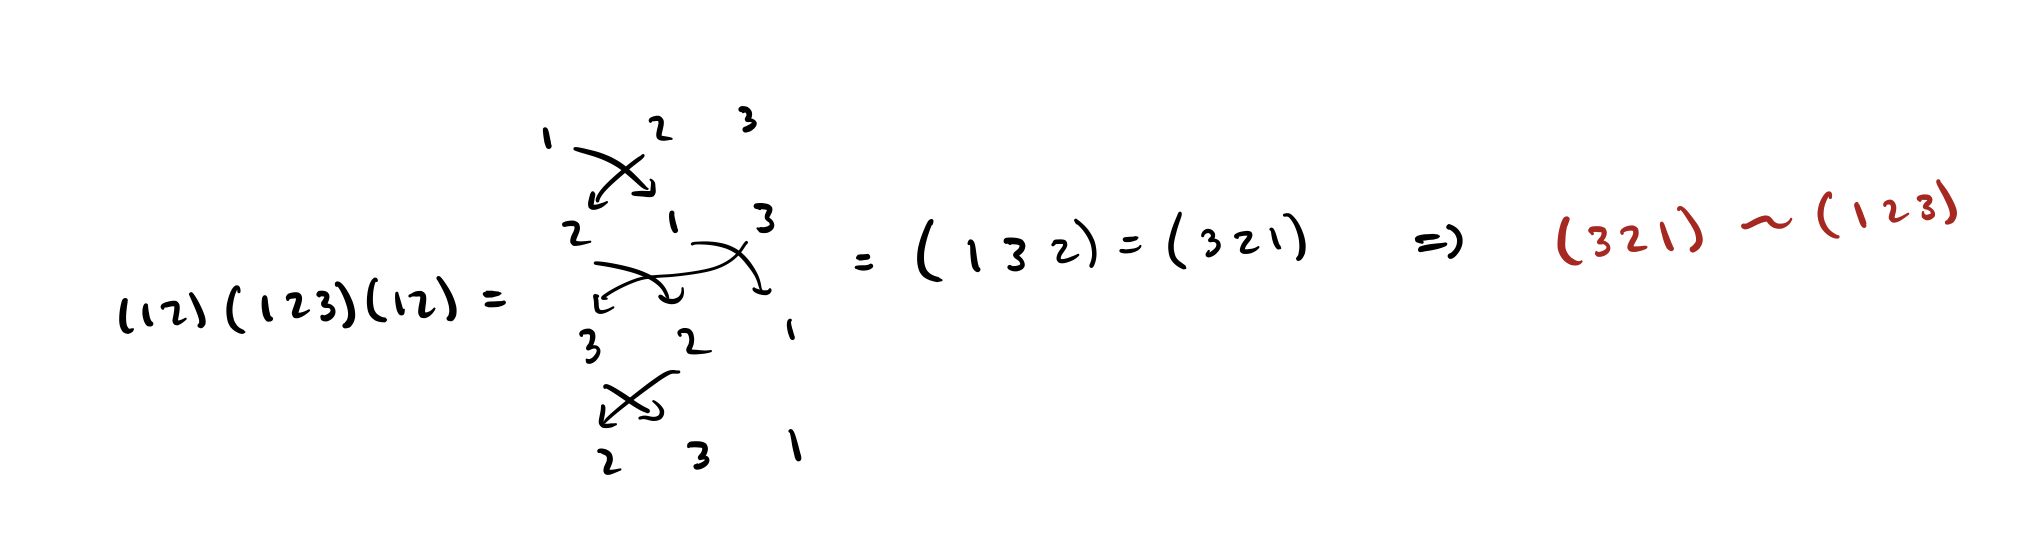
\includegraphics[width=0.95\textwidth]{img/123eq}
            \caption{Showing $(123) \sim (321)$}
            \label{fig:123eq}
        \end{figure}

        \begin{figure}[h]
            \centering
            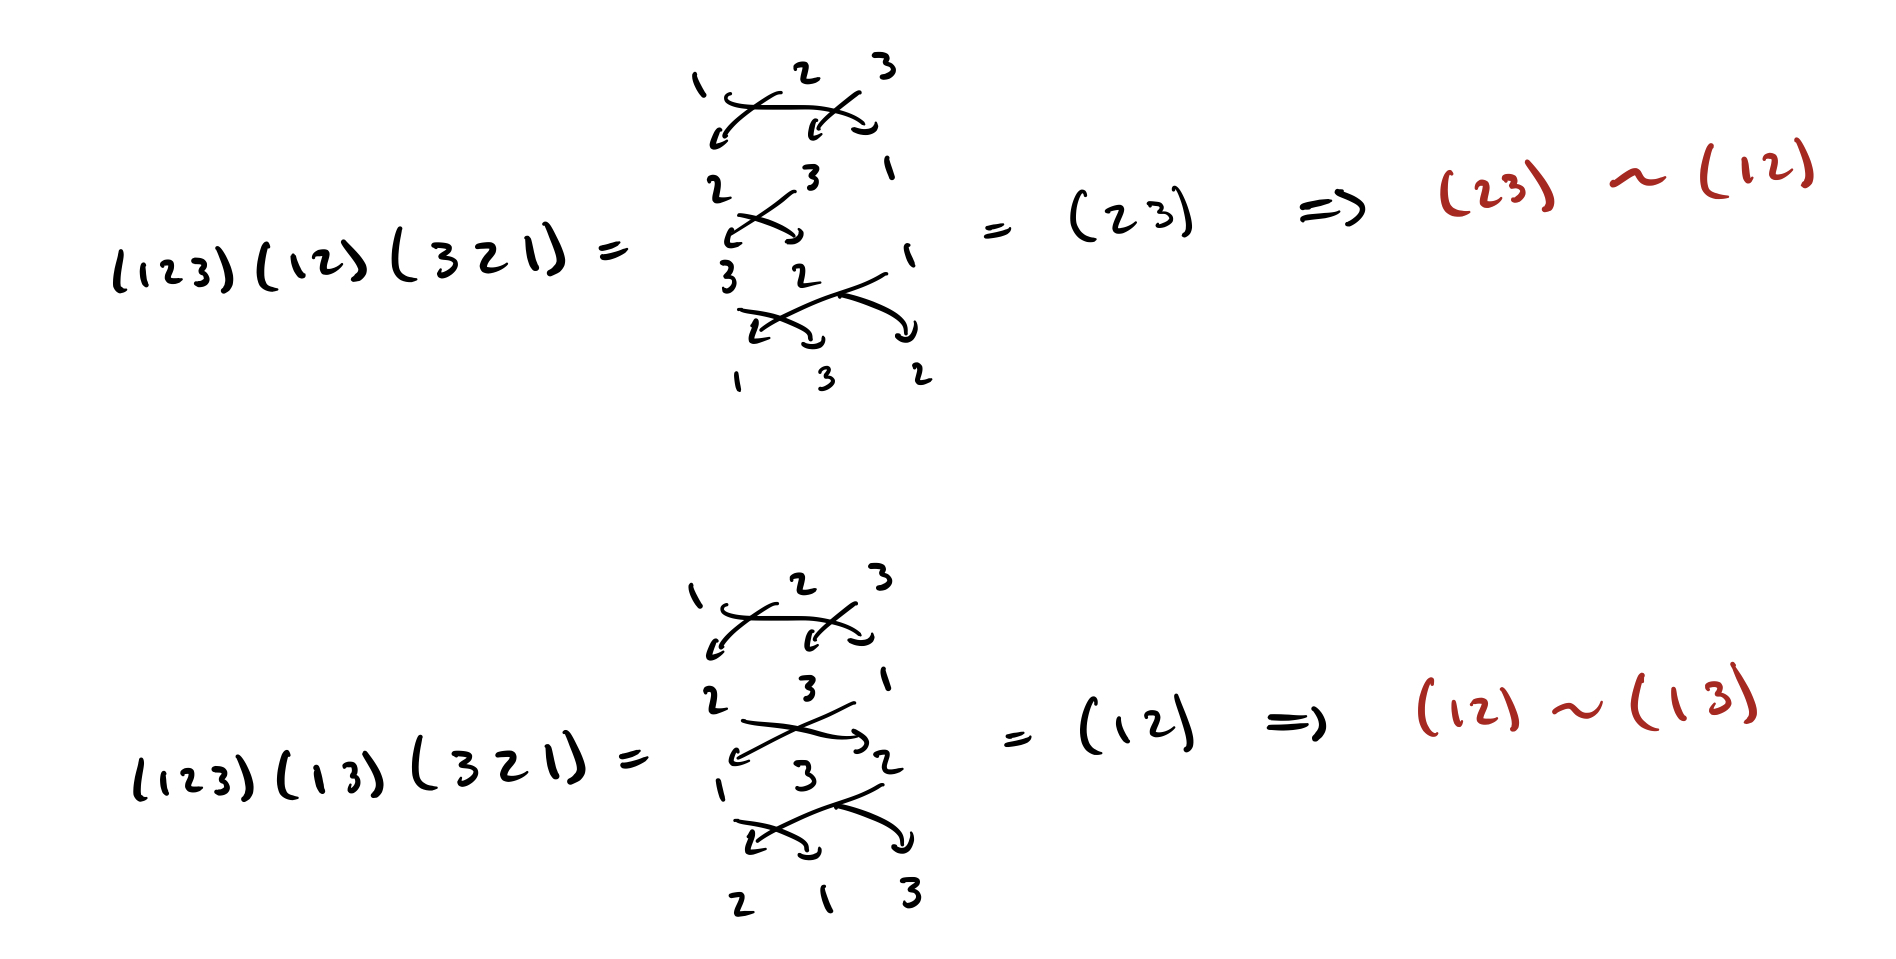
\includegraphics[width=0.85\textwidth]{img/12eq}
            \caption{Showing $(12) \sim (13) \sim (23)$}
            \label{fig:12eq}
        \end{figure}

        \newpage
        We now show that the conjugacy classes of $S_3$ are $A_1 = \{ id \}$, $A_2 = \{ (12), (13), (23) \}$, and $A_3 = \{ (123), (321) \}$.
        We already know $\{ id \}$ to be its own conjugacy class.
        So we only need show that $A_2, A_3$ are not part of the same conjugacy class.
        Since $\sim$ is an equivalence relation, it suffices to show that a single pair of elements from $A_2, A_3$ are not in the same conjugacy class.
        Can we show $(12)$ and $(123)$ are not in the same conjugacy class?
        Suppose $(12) \sim (123)$, then there exists $h \in G$ such that $(12) = h^{-1} (123) h$.
        Then it must also be true that $(12)^3 = (h^{-1} (123) h)^3$.
        Simplifying, $(12)^3 = (12)$ and $(h^{-1} (123) h)^3 = h^{-1} (123)^3 h = h^{-1} id h = h^{-1} h = id$.
        But $(12) \neq id$ so we have reached a contradiction and the elements $(12)$ and $(123)$ cannot be part of the same conjugacy class.
        Then their conjugacy classes must be distinct (since $\sim$ is an equivalence relation).
        Therefore the conjugacy classes o $S_3$ are $A_1 = \{ id \}$, $A_2 = \{ (12), (13), (23) \}$, and $A_3 = \{ (123), (321) \}$.
    }
\end{exercise}

% hw problem 3 -----------------------------------------------------------------

\begin{exercise}{65}{21}
    \problem{
        Let $G$ be the dihedral group of order 8.
        Find the conjugacy classes in $G$.
    }
    \proof{
    }
\end{exercise}

% hw problem 4 -----------------------------------------------------------------

\newpage
\section*{Heisenberg group problem}
    \problem{
        Find the center of our new friend, the Heisenberg group,
        $$ \H _3 (\R) :=
        \left\{
            \begin{bmatrix}
                1 & x & z \\
                0 & 1 & y \\
                0 & 0 & 1
            \end{bmatrix}
            \mid x,y,z \in \R
        \right\} $$
    }
    \proof{

    }

% hw problem 5 -----------------------------------------------------------------

\newpage
\section*{Crayon the clock}
    \problem{
        Let $G$ be equal to $\Z _{15} := \{ 0, 1, 2, ..., 14 \}$.
        Draw it some way.
        Find a subgroup $H$ of order $|H| = 5$ and then color differently all the different subsets of $\Z _{15}$ of the form $aH$.
        (How many are there?)
        If you have more crayons, do another drawing for an $H$ with $|H| = 3$.
    }
    \proof{

    }

\end{document}
